\documentclass[border=10pt]{standalone}
\usepackage{pgfplots}
\pgfplotsset{compat=1.18}
\usetikzlibrary{arrows.meta, shapes, calc}

\begin{document}

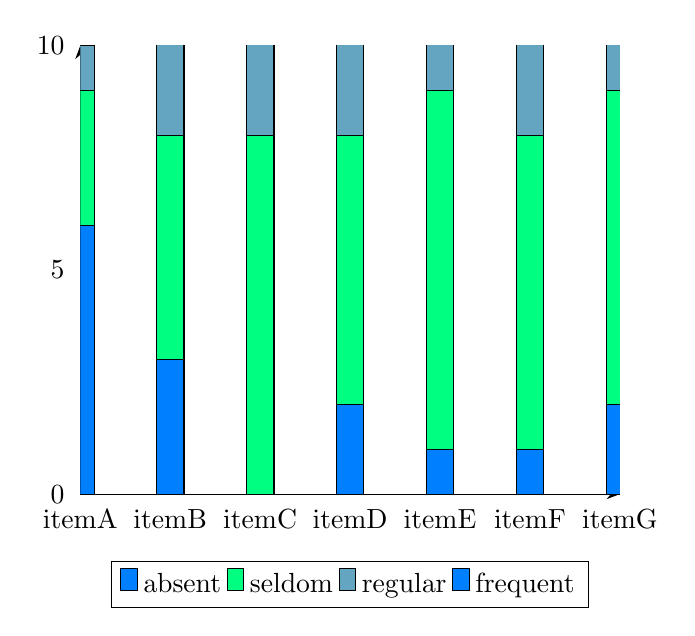
\begin{tikzpicture}
    \begin{axis}[
        ybar stacked,
        bar width=10pt,
        ymin=0, ymax=10,
        xtick=data,
        xticklabels={itemA, itemB, itemC, itemD, itemE, itemF, itemG},
        ytick={0,5,10},
        yticklabels={0, 5, 10},
        axis lines=left,
        axis line style={-Stealth},
        tick style={draw=none},
        legend style={at={(0.5,-0.15)}, anchor=north, legend columns=-1},
        nodes near coords,
        nodes near coords align={vertical},
        point meta=explicit symbolic,
        ]
        \addplot[fill=blue!50!cyan] coordinates {(1,6) (2,3) (3,0) (4,2) (5,1) (6,1) (7,2)};
        \addplot[fill=green!50!cyan] coordinates {(1,3) (2,5) (3,8) (4,6) (5,8) (6,7) (7,7)};
        \addplot[fill=gray!50!cyan] coordinates {(1,1) (2,9) (3,8) (4,6) (5,2) (6,7) (7,7)};
        \addplot[fill=blue!50!cyan] coordinates {(1,9) (2,10) (3,10) (4,10) (5,8) (6,10) (7,10)};
        \legend{absent, seldom, regular, frequent}
    \end{axis}
\end{tikzpicture}

\end{document}